\documentclass{lastenheft}
\usepackage{glossaries}

\setauthor{Patrick Gustav Blaneck} % Autor hier
\title{Fahrkartenautomat Lastenheft \\ (Requirements-Specification)}

\makenoidxglossaries 

%\newglossaryentry{glos:ausgabeschacht}{
%    name=Ausgabeschacht,
%    description={kacke}
%}

%\newglossaryentry{glos:auswahltasten}
%{
%    name=Auswahltasten,
%    description={pisse}
%}

%\newglossaryentry{glos:abbruchtaste}
%{
%    name=Abbruch-Taste,
%    description={arsch}
%}

\newglossaryentry{glos:betrag}
{
    name=Betrag,
    description={ der (Geld-)Betrag, der Gegenstand des Zahlungsvorgangs (Valutaverhältnis) ist, welcher also überwiesen (Überweisung), per Lastschrift eingezogen oder per Zahlungskarte bezahlt werden soll}
}

\newglossaryentry{glos:muenzspeicher}
{
    name=Münzspeicher,
    description={Behältnis für alle aus Metall hergestellten, scheibenförmigen Geldstücke von bestimmtem Gewicht und Feingehalt und mit beidseitigem Gepräge}
}

\newglossaryentry{glos:software}
{
    name=Software,
    description={beschreibt sämtliche nicht physische Bestandteile eines Computers, Computernetzwerks oder mobilen Geräts. Gemeint sind die Programme und Anwendungen (wie das Betriebssystem), die den Computer für den Nutzer funktionstüchtig machen}
}

\newglossaryentry{glos:fahrkarte}
{
    name=Fahrkarte,
    description={kleine Karte, die (gegen Entrichtung eines bestimmten Geldbetrags) zum Fahren mit einem öffentlichen Verkehrsmittel berechtigt}
}

\newglossaryentry{glos:benutzeroberflaeche}
{
    name=Benutzeroberfläche,
    description={auf dem Bildschirm eines Computers sichtbare Darstellung eines Programms}
}

\newglossaryentry{glos:kaufvorgang}
{
    name=Kaufvorgang,
    description={gegenseitiger, i.d.R. formlos wirksamer Vertrag, durch den sich der Verkäufer zur Übertragung (des Eigentums und des Besitzes) eines Gegenstandes (Sache oder Recht) an den Käufer und dieser sich zur Zahlung des vereinbarten Kaufpreises an den Verkäufer (und zur Abnahme der Kaufsache) verpflichtet}
}

\newglossaryentry{glos:fernzugriff}
{
    name=Fernzugriff,
    description={bezeichnet den Zugriff auf technische Anlagen über eine räumliche Distanz hinweg}
}

\newglossaryentry{glos:protokoll}
{
    name=Protokoll (\textmd{auch} protokollieren),
    text=Protokoll,
    description={genauer Bericht über Verlauf und Ergebnis eines Versuchs, einer Operation o. Ä.}
}

\newglossaryentry{glos:protokollieren}
{
    name=protokollieren,
    description={\emph{Siehe} \gls{glos:protokoll}}
}

\newglossaryentry{glos:softwareversion}
{
    name=Softwareversion,
    description={ ist ein definiertes Entwicklungsstadium einer Software mit allen dazugehörigen Komponenten}
}

\newglossaryentry{glos:wartung}
{
    name=Wartung,
    description={ Instandhaltung von etwas durch entsprechende Pflege, regelmäßige Überprüfung und Ausführung notwendiger Reparaturen}
}

\newglossaryentry{glos:betriebsmittel}
{
    name=Betriebsmittel,
    description={als elementare Produktionsfaktoren verstanden, die langfristig zum Einsatz kommen und für den Herstellungsprozess erforderlich sind. \emph{Hier} Papier, Farbbänder, Münzen}
}

\newglossaryentry{glos:transaktion}
{
    name=Transaktion,
    description={bezieht sich auf den Tausch von Waren und Dienstleistungen gegen andere Güter oder gegen Geld}
}

\newglossaryentry{glos:stornierung}
{
    name=Stornierung,
    description={Rückziehung eines Auftrages}
}

\newglossaryentry{glos:leichtesprache}
{
    name=Leichte Sprache,
    description={speziell geregelte einfache Sprache. Die sprachliche Ausdrucksweise des Deutschen zielt dabei auf die besonders leichte Verständlichkeit}
}

\newglossaryentry{glos:zahlungsmethode}
{
    name=Zahlungsmethode (\textmd{auch} Zahlungsart),
    text=Zahlungsmethode,
    description={ermöglichen im alltäglichen und wirtschaftlichen Leben den Übertrag von finanziellen Mitteln, welche im Zuge eines Kaufgeschäfts vom Käufer auf den Verkäufer weitergegeben werden}
}

\newglossaryentry{glos:zahlungsschnittstelle}
{
    name=Zahlungsschnittstelle,
    description={etwasm womit man bezahlen kann}
}

\newglossaryentry{glos:angebot}
{
    name=Angebot (\textmd{auch} Sonderangebot),
    text=Angebot,
    description={auf eine kurze Zeitspanne beschränktes preiswertes Angebot einer Ware}
}

\newglossaryentry{glos:rueckgeld}
{
    name=Rückgeld,
    description={Differenz zwischen zu zahlendem Betrag und tatsächlich gegebenem Betrag bei einer Barzahlung, die man in bar umgehend zurückerstattet bekommt}
}

\newglossaryentry{glos:barzahlung}
{
    name=Barzahlung,
    description={Zahlungsform, bei der der Schuldner dem Gläubiger Bargeld übergibt}
}

\newglossaryentry{glos:bargeldlosezahlung}
{
    name=Bargeldlose Zahlung,
    description={Abwicklung von Zahlungen ohne Verwendung von Bargeld}
}

\newglossaryentry{glos:dunkelmodus}
{
    name=Dunkelmodus,
    description={ist eine Benutzeroberfläche (UI) für Inhalte, die hellen Text auf dunklem Hintergrund anzeigt}
}

\newglossaryentry{glos:oled}
{
    name=OLED (\textmd{auch} organische Leuchtdiode),
    text=OLED,
    description={ist ein leuchtendes Dünnschichtbauelement aus organischen halbleitenden Materialien, das sich von den anorganischen Leuchtdioden (LED) dadurch unterscheidet, dass die elektrische Stromdichte und Leuchtdichte geringer und keine einkristallinen Materialien erforderlich sind. Im Vergleich zu herkömmlichen (anorganischen) Leuchtdioden lassen sich organische Leuchtdioden daher in Dünnschichttechnik kostengünstiger herstellen}
}

\newglossaryentry{glos:datentransfer}
{
    name=Datentransfer,
    description={der elektronische Transport von Daten }
}

\newglossaryentry{glos:passwortrichtlinie}
{
    name=Passwortrichtlinie,
    description={stellen Vorgaben dar, an welche man Benutzer binden kann – man erzwingt sozusagen den Einsatz von Passwörtern einer bestimmten Komplexität}
}

\newglossaryentry{glos:identitymanagement}
{
    name={Identity Management (\textmd{auch} Identitäts-Management, ID-Management)},
    text=Identity Management,
    description={Oberbegriff für die Prozesse innerhalb einer Organisation, die sich mit der Verwaltung und Pflege von Benutzerkonten und Ressourcen im Netzwerk befassen, einschließlich der Berechtigungsverwaltung für Benutzer auf Anwendungen und Systeme}
}

\begin{document}
\maketitle

\tableofcontents

\section{Historie}
\begin{tabularx}{\textwidth}{|l|l|X|}
    \hline
    \textbf{Datum} & \textbf{Name}          & \textbf{Beschreibung}  \\
    \hline
    23.10.2021     & Patrick Gustav Blaneck & Erste Version erstellt \\
    \hline
    24.10.2021     & Patrick Gustav Blaneck & Anwendungsfalldiagramm \\
    \hline
    25.10.2021     & Patrick Gustav Blaneck & 1.0 fertiggestellt     \\
    \hline
                   &                        &                        \\
    \hline
                   &                        &                        \\
    \hline
                   &                        &                        \\
    \hline
                   &                        &                        \\
    \hline
                   &                        &                        \\
    \hline
                   &                        &                        \\
    \hline
                   &                        &                        \\
    \hline
                   &                        &                        \\
    \hline
\end{tabularx}

\newpage

\section{Stakeholder und Ziele}

Stakeholder sind:
\begin{itemize}
    \item \nameref{sec:PrivatkundInnen}
    \item \nameref{sec:Verkehrsbetriebe}
    \item \nameref{sec:Administration}
    \item \nameref{sec:Servicepersonal}
    \item \nameref{sec:Finanzdienstleistende}
\end{itemize}

\subsection*{PrivatkundInnen}
\label{sec:PrivatkundInnen}
Zu entwickeln ist die \gls{glos:software} für einen Fahrkartenautomaten.
Ein Fahrkartenautomat dient dem Verkauf von \gls{glos:fahrkarte}n an \emph{PrivatkundInnen}.
Dabei sollen \gls{glos:benutzeroberflaeche} und \gls{glos:kaufvorgang} intuitiv und simpel gestaltet werden.
Der Kunde kann den \gls{glos:kaufvorgang} jederzeit abbrechen.

\subsection*{Verkehrsbetriebe}
\label{sec:Verkehrsbetriebe}
Die Betreibenden der Automaten - die \emph{Verkehrsbetriebe} - haben ein Interesse daran, dass die Entwicklungs-, Weiterentwicklungs- und Instandhaltungskosten effektiv genutzt werden.
Die \gls{glos:software} der Fahrkartenautomaten soll weiterhin eine positive Außenwirkung erzielen.
Sie stellt einen unabdingbaren Teil des Portfolios der Dienstleistungen der Verkehrsbetriebe dar.

\subsection*{Administration}
\label{sec:Administration}
Die \emph{Administration} der Verkehrsbetriebe muss per \gls{glos:fernzugriff} den Automaten warten und deaktivieren können; dazu ist ein jeder Fahrkartenautomat mit dem Server der Verkehrsbetriebe vernetzt.
Nach erfolgter Anmeldung erhalten sie Einsicht über \gls{glos:protokoll}e, den aktuellen \gls{glos:muenzspeicher} und die \gls{glos:softwareversion}.

\subsection*{Servicepersonal}
\label{sec:Servicepersonal}
Das \emph{Servicepersonal} muss in der Lage sein sowohl auf Abruf als auch auf Eigeninitiative hin \gls{glos:wartung}en am Fahrkartenautomaten durchführen zu können.
Um vermeidbaren Mehraufwand zu minimieren, sollen routinemäßige Kontrollen, verbunden mit der Versorgung mit \gls{glos:betriebsmittel}n (z.B. Papier, Farbbänder), durchgeführt werden.
Dadurch werden etwaige Notfälle auf das Nötigste reduziert.

\subsection*{Finanzdienstleistende}
\label{sec:Finanzdienstleistende}
Für bargeldlose \gls{glos:transaktion}en ist Kooperation mit diversen \emph{Finanzdienstleistenden} nötig.
Diese fordern geregelte Zahlungstransaktionsprozesse und potentiell Anteile an jeder \gls{glos:transaktion}, welche transparent kommuniziert werden müssen.
Im Zuge der Digitalisierung sollen bargeldlose \gls{glos:transaktion}en bevorzugt dargestellt werden.

\section{Anwendungsfalldiagramm}

\makebox[\textwidth][c]{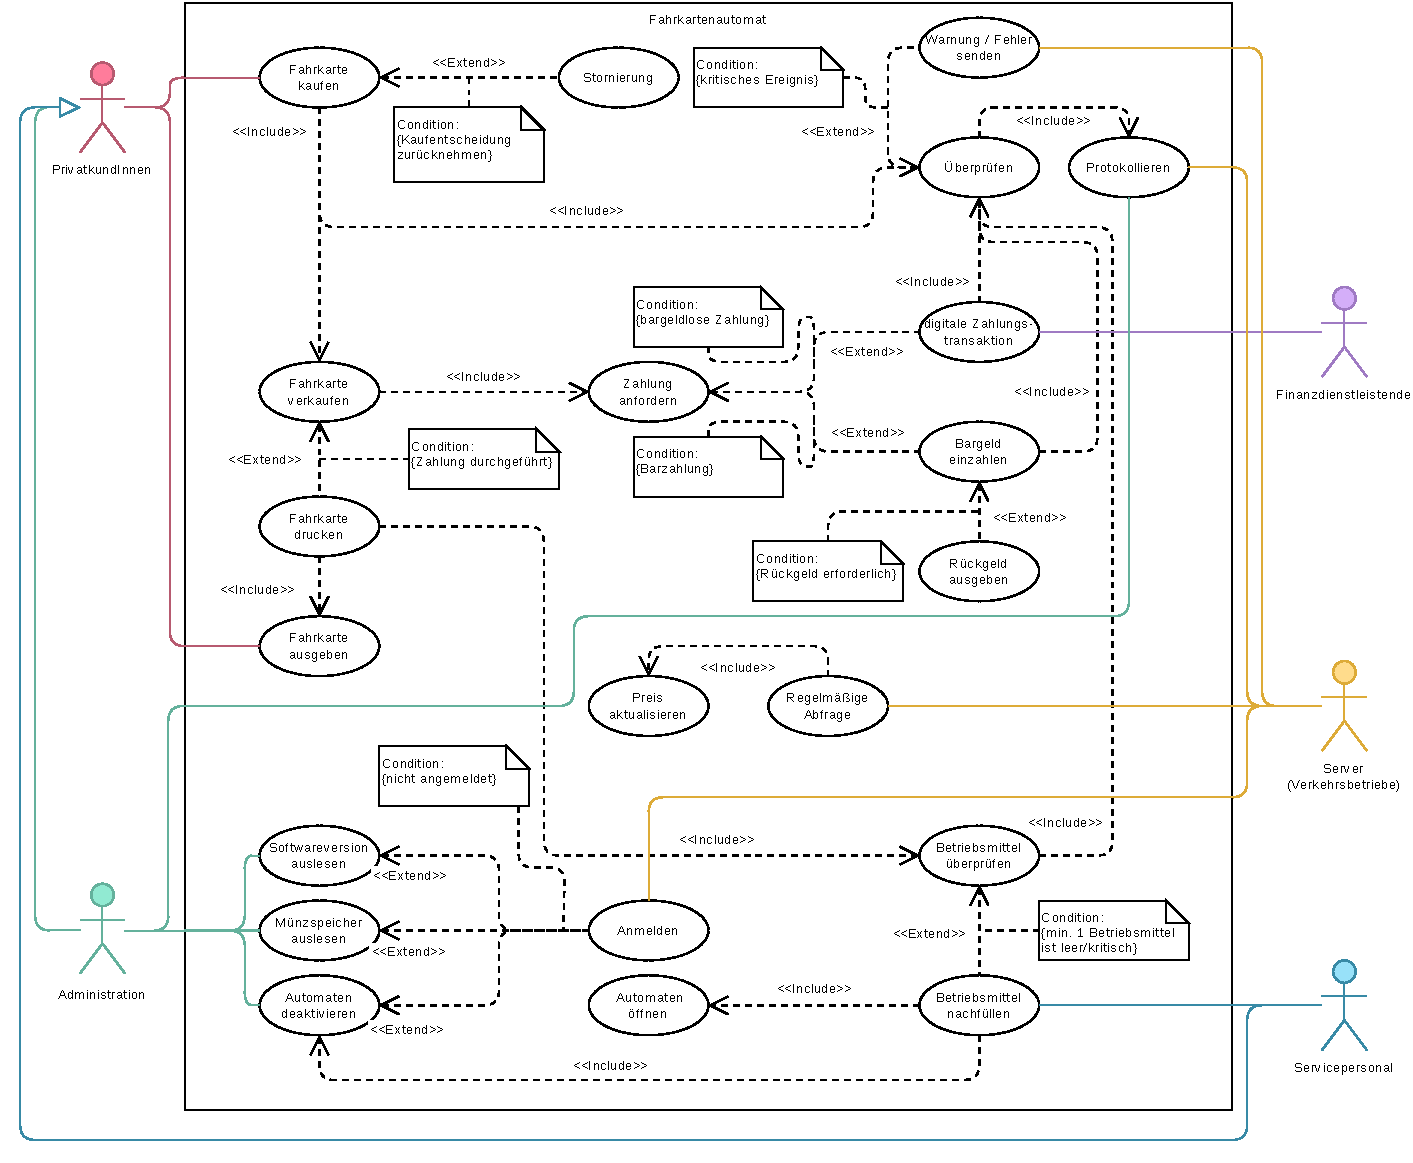
\includegraphics[width=1.7\textwidth]{use_case.pdf}}%

%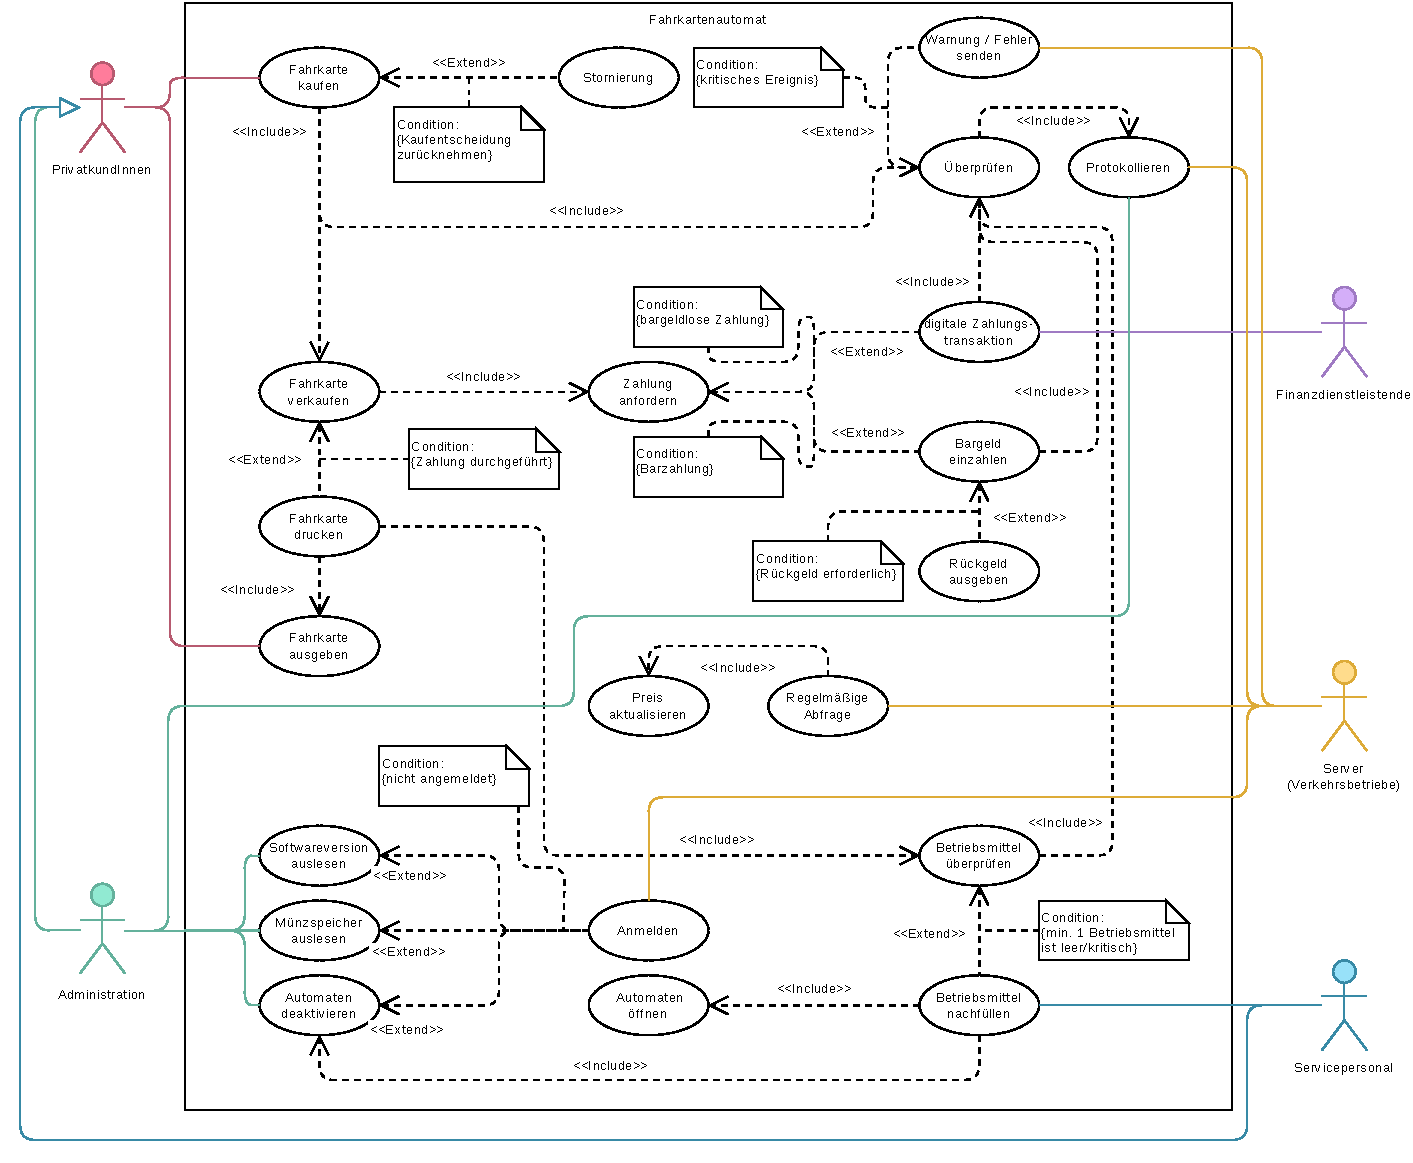
\includegraphics[width=\textwidth]{use_case.pdf}
%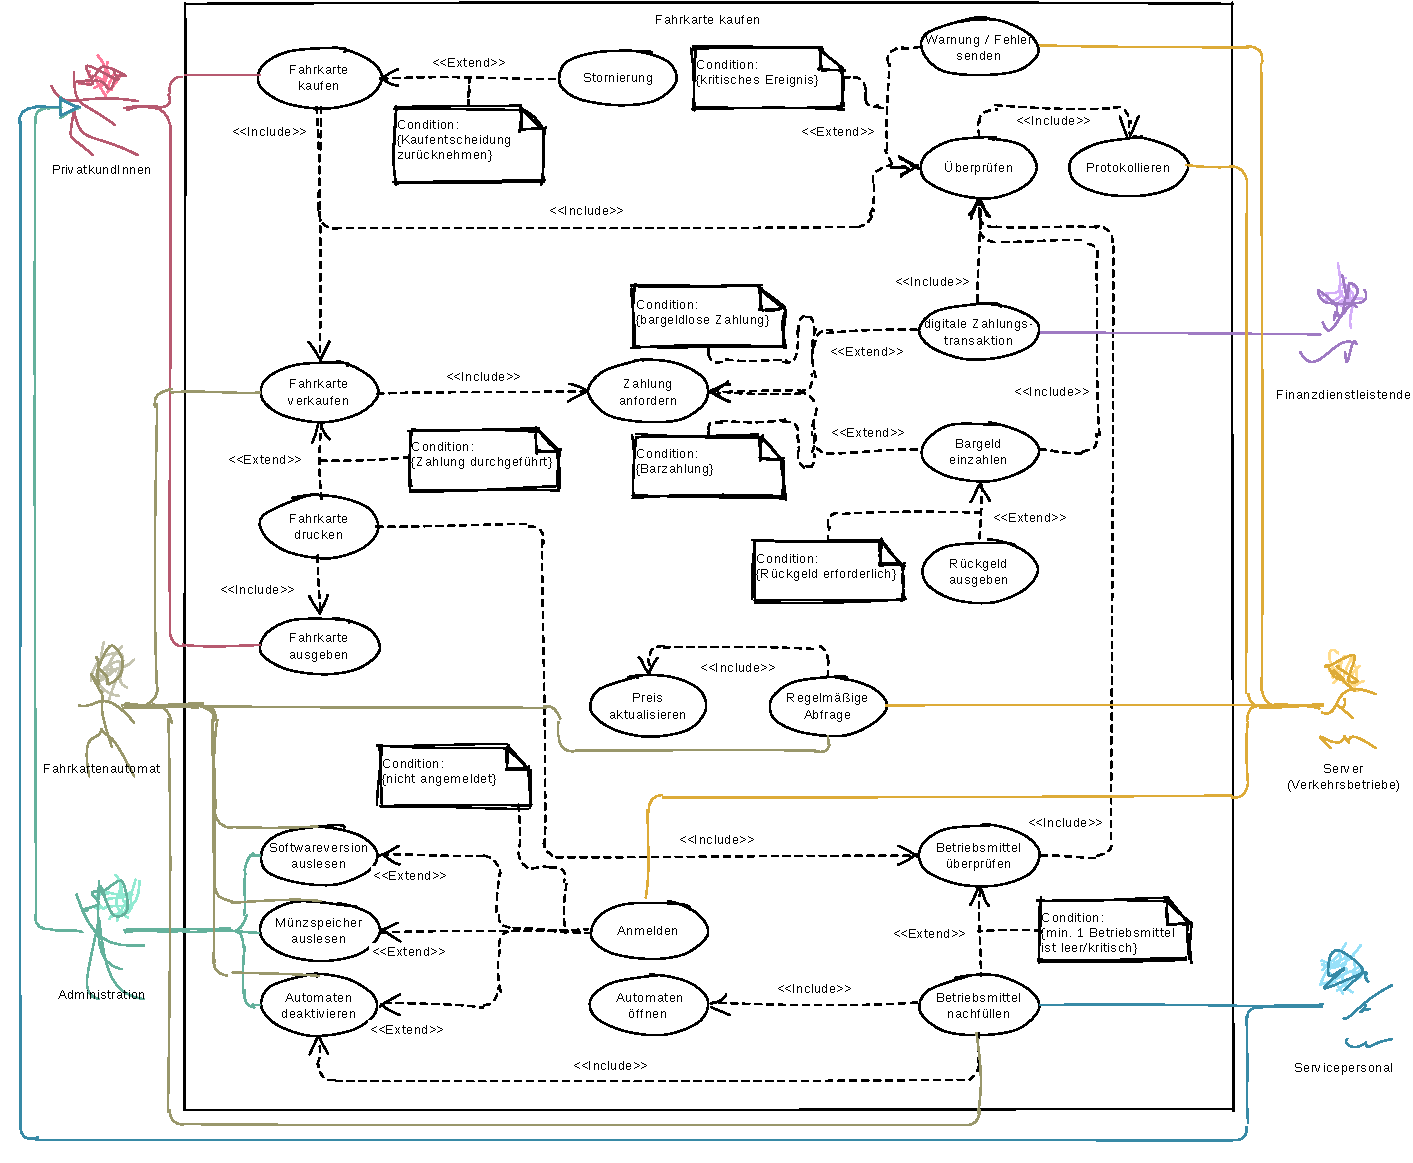
\includegraphics[width=\textwidth]{use_case_scuffed.pdf}

%Im Anhang befindet sich eine größere Version des Anwendungsfalldiagramms.

\clearpage

\section{Anwendungsfälle}
\subsection{Fahrkahrte kaufen}

\begin{xltabular}{\linewidth}{|>{\bfseries}p{4cm}|X|}
    \hline
    Name des Use Cases & \gls{glos:fahrkarte} kaufen \\
    \hline
    Nummer & UC1 \\
    \hline
    AutorIn & Patrick Gustav Blaneck \\
    \hline
    Version & 0.1 Patrick Gustav Blaneck: Erste Erstellung \\
    \hline
    Kurzbeschreibung & Der Anwendungsfall beschreibt den Fahrkartenverkauf durch einen Kunden der Verkehrsbetriebe.\\
    \hline
    beteiligte Aktoren & - PrivatkundInnen \\
    (Stakeholder) & - Verkehrsbetriebe \\
    & - Finanzdienstleistende \\
    \hline
    Referenzen & - Einbeziehen der Steuer \\
    & - Fremdsprachenauswahl \\
    & - Option für \gls{glos:leichtesprache} \\
    & - Abfragen der \gls{glos:zahlungsmethode}n \\
    & - Abrufen verfügbarer \gls{glos:fahrkarte}n \\
    & - Aktuelle \gls{glos:angebot}e anzeigen \\
    \hline
    Vorbedingungen & - Fahrkartenautomat arbeitet ordnungsgemäß \\
    & - \gls{glos:betriebsmittel} sind ausreichend verfügbar \\
    \hline
    Nachbedingungen & - potent. \gls{glos:rueckgeld} wurde korrekt behandelt \\
    & - potent. Kommunikation mit Finanzdienstleistenden wurde ordnungsgemäß beendet \\
    & - \gls{glos:fahrkarte} wurde gedruckt und entnommen \\
    \hline
    typischer Ablauf & 1. Privatkunde/-in initialisiert \gls{glos:kaufvorgang} \\
    & 2. Fahrkartenautomat beginnt Verkaufsvorgang \\
    & 3. Zahlung wird angefordert \\
    & 4. Kunde wählt \gls{glos:barzahlung} \\
    & 5. Kunde zahlt Bargeld ein \\
    & 6. Fahrkartenautomat gibt, falls nötig, \gls{glos:rueckgeld} \\
    & 7. Fahrkartenautomat druckt Fahrkahrte \\
    & 8. \gls{glos:fahrkarte} wird ausgegeben und entnommen \\
    \hline
    alternative Abläufe & \textbf{\gls{glos:bargeldlosezahlung}} \\
    & 1. Privatkunde/-in initialisiert \gls{glos:kaufvorgang} \\
    & 2. Fahrkartenautomat beginnt Verkaufsvorgang \\
    & 3. Zahlung wird angefordert \\
    & 4. Kunde wählt \gls{glos:bargeldlosezahlung} \\
    & 5. Verbindung sich mit Finanzdienstleistenden \\
    & 6. Fahrkartenautomat fordert etwaige Eingaben \\
    & 7. Privatkunde/-in vollzieht \gls{glos:transaktion} \\
    & 8. Fahrkartenautomat druckt Fahrkahrte \\
    & 9. \gls{glos:fahrkarte} wird ausgegeben und entnommen \\
    %\newpage
    & \textbf{Beenden wegen Inaktivität} \\
    & 1. Privatkunde/-in initialisiert  \gls{glos:kaufvorgang} \\
    & 2. An beliebigem Zeitpunkt im \gls{glos:kaufvorgang} ist Privatkunde/-in 2 Minuten inaktiv \\
    & 3. Fahrkartenautomat führt \gls{glos:stornierung} durch \\
    \hline
    Kritikalität & Sehr Hoch; Essentielle Funktionalität\\
    \hline
    Verknüpfungen & UC2: Vorgänge \gls{glos:protokollieren} \\
    & UC4: \gls{glos:betriebsmittel} nachfüllen \\
    \hline
    funktionale & siehe Text.\\
    Anforderungen & E: Fahrkartenauswahl \\
    & A: \gls{glos:betrag} \\
    & E: \gls{glos:zahlungsmethode} \\
    & E: Relevante Daten \\
    & (A: \gls{glos:rueckgeld}) \\
    & A: \gls{glos:fahrkarte} \\
    \hline
    nicht-funktionale & - Anpassen der Anzeigesprache \\
    Anforderungen & - \gls{glos:dunkelmodus} verbunden mit \gls{glos:oled}-Displays zum Energiesparen \\
    & - Nutzung diversester \gls{glos:zahlungsmethode}n und -schnittstellen \\
    & - Senden einer Rechnung per Mail \\
    \hline
\end{xltabular}

\subsection{Münzspeicher auslesen}

\begin{xltabular}{\linewidth}{|>{\bfseries}p{4cm}|X|}
    \hline
    Name des Use Cases & \gls{glos:muenzspeicher} auslesen \\
    \hline
    Nummer & UC3 \\
    \hline
    AutorIn & Patrick Gustav Blaneck \\
    \hline
    Version & 0.1 Patrick Gustav Blaneck: Erste Erstellung \\
    \hline
    Kurzbeschreibung & Der Anwendungsfall beschreibt das Auslesen des aktuellen \gls{glos:muenzspeicher}s durch die Administration.\\
    \hline
    beteiligte Aktoren & - Administration \\
    (Stakeholder) & - Verkehrsbetriebe \\
    \hline
    Referenzen & - Verschlüsselter \gls{glos:datentransfer} \\
    & - Stabile Internetverbindung \\
    & - \gls{glos:passwortrichtlinie}n \\
    & - Ausloggen bei Inaktivität \\
    & - Freischalten neuer Administrierenden \\
    \hline
    Vorbedingungen & - Fahrkartenautomat arbeitet ordnungsgemäß \\
    & - existentes \gls{glos:identitymanagement} \\
    & - funktionierende Verbindung zum Server \\
    & - Administration kennt Zugangsdaten \\
    & - Status des \gls{glos:muenzspeicher}s wird korrekt erfasst \\
    \hline
    Nachbedingungen & - Administration hat Informationen zum \gls{glos:muenzspeicher} erhalten \\
    \hline
    %\newpage
    typischer Ablauf & 1. Administration möchte \gls{glos:muenzspeicher} auslesen \\
    & 2. Administration loggt sich über das \gls{glos:identitymanagement} der Verkehrsbetriebe auf dem Fahrkartenautomaten ein \\
    & 3. Administration kann \gls{glos:muenzspeicher} auslesen \\
    & 4. Administration loggt sich aus \\
    \hline
    alternative Abläufe & \textbf{Inaktivität} \\
    & 1. Administration möchte \gls{glos:muenzspeicher} auslesen \\
    & 2. Administration loggt sich über das \gls{glos:identitymanagement} der Verkehrsbetriebe auf dem Fahrkartenautomaten ein \\
    & 3. Administration ist inaktiv \\
    & 4. Administration wird ausgeloggt \\
    \hline
    Kritikalität & Mittel; durch routinemäßige Kontrollen nur in Ausnahmefällen problematisch\\
    \hline
    Verknüpfungen & UC2: Vorgänge \gls{glos:protokollieren} \\
    \hline
    funktionale & siehe Text. \\
    Anforderungen & E: URL zum Auslesen des \gls{glos:muenzspeicher}s \\
    & A: Eingabefeld für Zugangsdaten \\
    & E: gültige Zugangsdaten \\
    & A: Zugang zu Informationen des \gls{glos:muenzspeicher} des Fahrkartenautomaten \\
    \hline
    nicht-funktionale & - Anpassen der Anzeigesprache \\
    Anforderungen & - Export des Status des \gls{glos:muenzspeicher}s \\
    & - Zugangsdaten neu generieren lassen \\
    & - Neue administrierende Personen anlegen  \\
    \hline
\end{xltabular}

\subsection{\gls{glos:betriebsmittel} nachfüllen}

\begin{xltabular}{\linewidth}{|>{\bfseries}p{4cm}|X|}
    \hline
    Name des Use Cases & \gls{glos:betriebsmittel} nachfüllen \\
    \hline
    Nummer & UC4 \\
    \hline
    AutorIn & Patrick Gustav Blaneck \\
    \hline
    Version & 0.1 Patrick Gustav Blaneck: Erste Erstellung \\
    \hline
    Kurzbeschreibung & Der Anwendungsfall beschreibt das Nachfüllen der \gls{glos:betriebsmittel} durch Servicepersonal.\\
    \hline
    beteiligte Aktoren & Servicepersonal\\
    (Stakeholder) & \\
    \hline
    Referenzen & - einheitliche \gls{glos:betriebsmittel} \\
    & - Inventarisierung aller \gls{glos:betriebsmittel} \\
    \hline
    Vorbedingungen & - Servicepersonal hat Zugangsmöglichkeit (z.B. Schlüssel) \\
    & - Fahrkartenautomat lässt sich auch im Notfall öffnen \\
    & - neue \gls{glos:betriebsmittel} sind vorhanden \\
    \hline
    Nachbedingungen & - \gls{glos:betriebsmittel} im Fahrkartenautomat sind ausreichend vorhanden \\
    \hline
    typischer Ablauf & 1. Servicepersonal erhält Zugang zum Fahrkartenautomaten \\
    & 2. Servicepersonal schaltet Fahrkartenautomaten ab \\
    & 3. unzureichend befüllte \gls{glos:betriebsmittel} werden nachgefüllt \\
    & 4. Fahrkartenautomat wird eingeschalten \\
    \hline
    alternative Abläufe & \textbf{Zugang blockiert} \\
    & physischer Zugang zum Fahrkartenautomaten ist blockiert durch externe Einflüsse \\
    \hline
    Kritikalität & Hoch; \gls{glos:betriebsmittel} sollten immer nachgefüllt werden können \\
    \hline
    Verknüpfungen & UC2: Vorgänge \gls{glos:protokollieren} \\
    \hline
    funktionale & siehe Text. \\
    Anforderungen & E: Möglichkeit des physischen Zugangs \\
    & E: Möglichkeit der Deaktivierung \\
    & A: Darstellen der Status der \gls{glos:betriebsmittel} vor Ort \\
    & A: Überprüfung der neuen \gls{glos:betriebsmittel} \\
    \hline
    nicht-funktionale & - Anpassen der Anzeigesprache \\
    Anforderungen & - Eigene \gls{glos:protokoll}e verfassen \\
    \hline
\end{xltabular}

\section{Nichtfunktionale Anforderungen}

\begin{enumerate}[font={\bfseries},label={NFRQ\arabic*:}]
    \item Anpassen der Anzeigesprache
    \item Implementierung verschiedenster \gls{glos:zahlungsmethode}n
    \item Implementierung verschiedenster \gls{glos:zahlungsschnittstelle}n
    \item Ansprechende grafische Oberflächen
\end{enumerate}

\subsection{Grafisches User Interface (Adminsicht)}
\makebox[\textwidth][c]{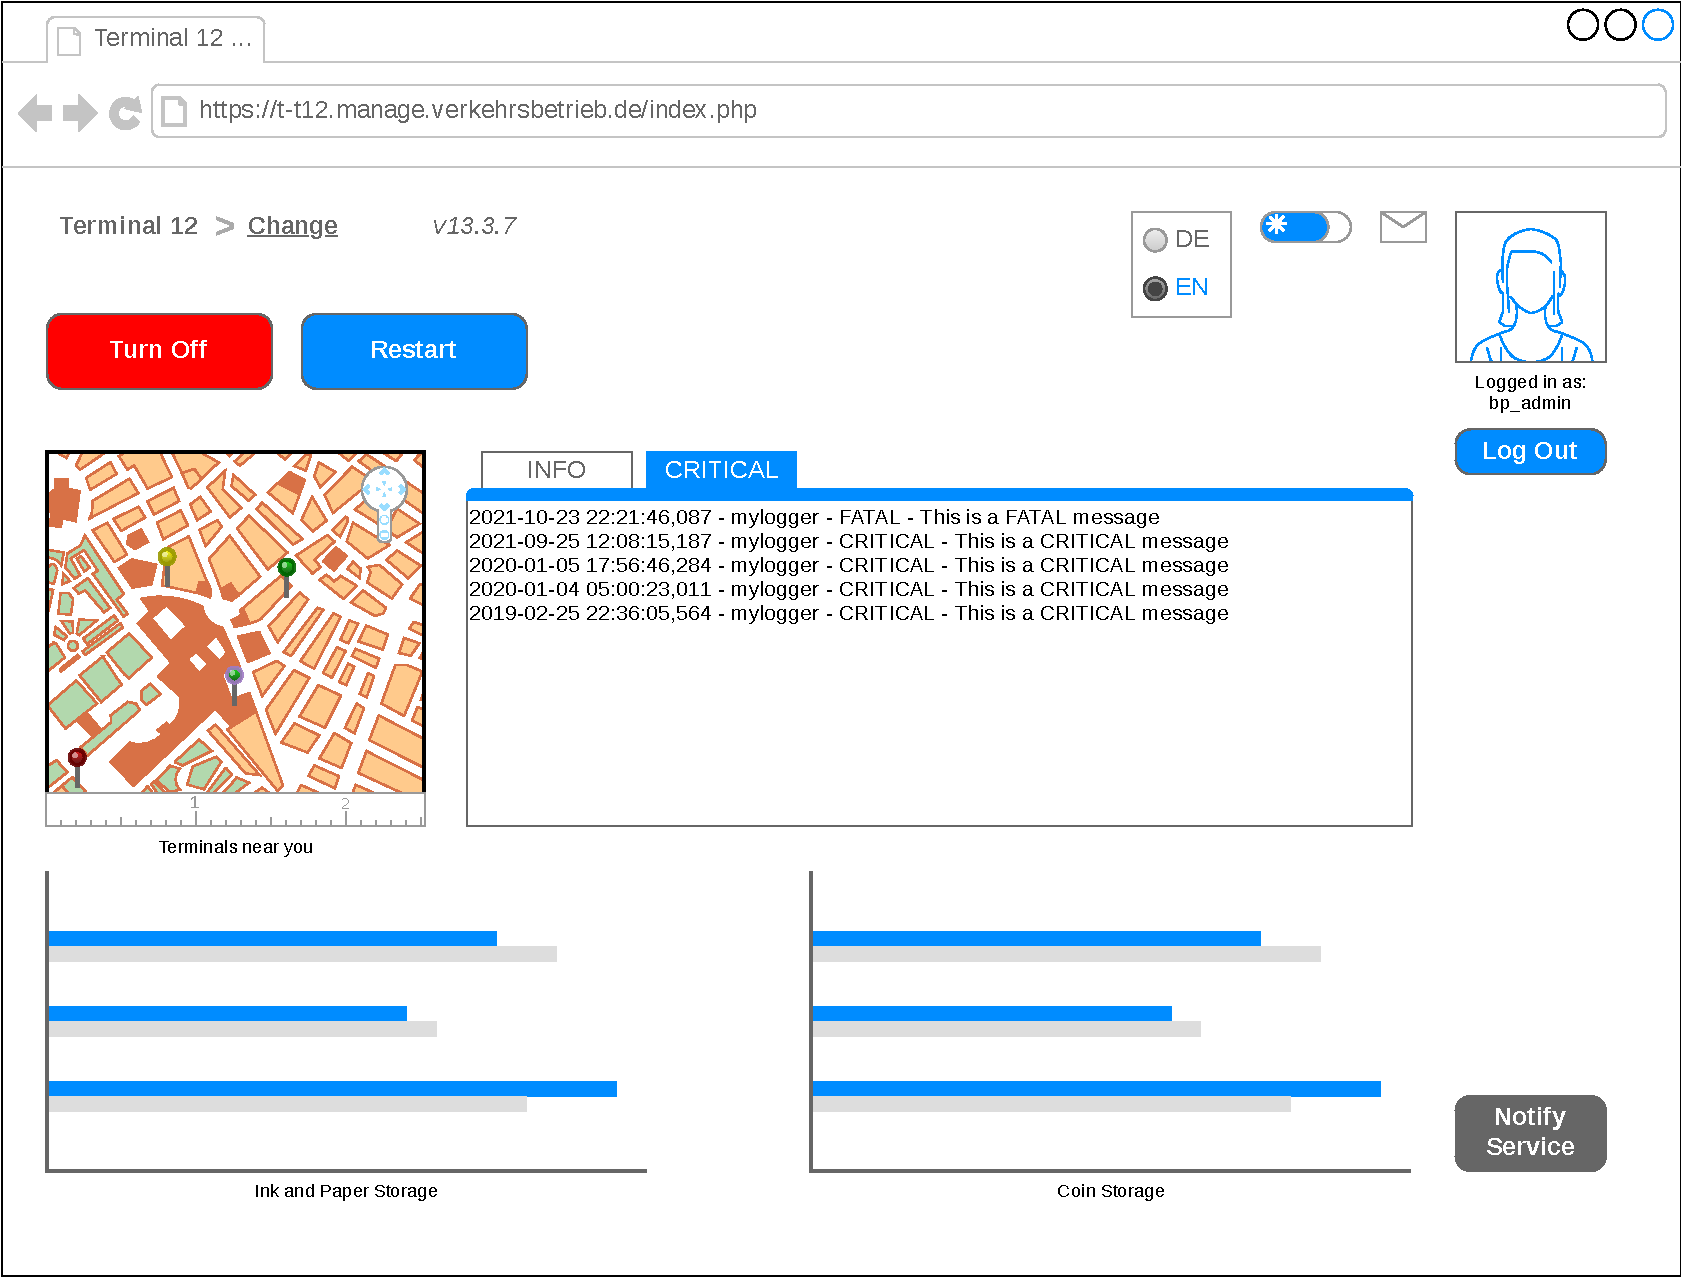
\includegraphics[width=1.2\textwidth]{mock.pdf}}%


\clearpage

\printnoidxglossaries
\addcontentsline{toc}{section}{Glossar}

\clearpage
%\begin{appendices}
%\section{Anwendungsfalldiagramm}
%\makebox[\textwidth][c]{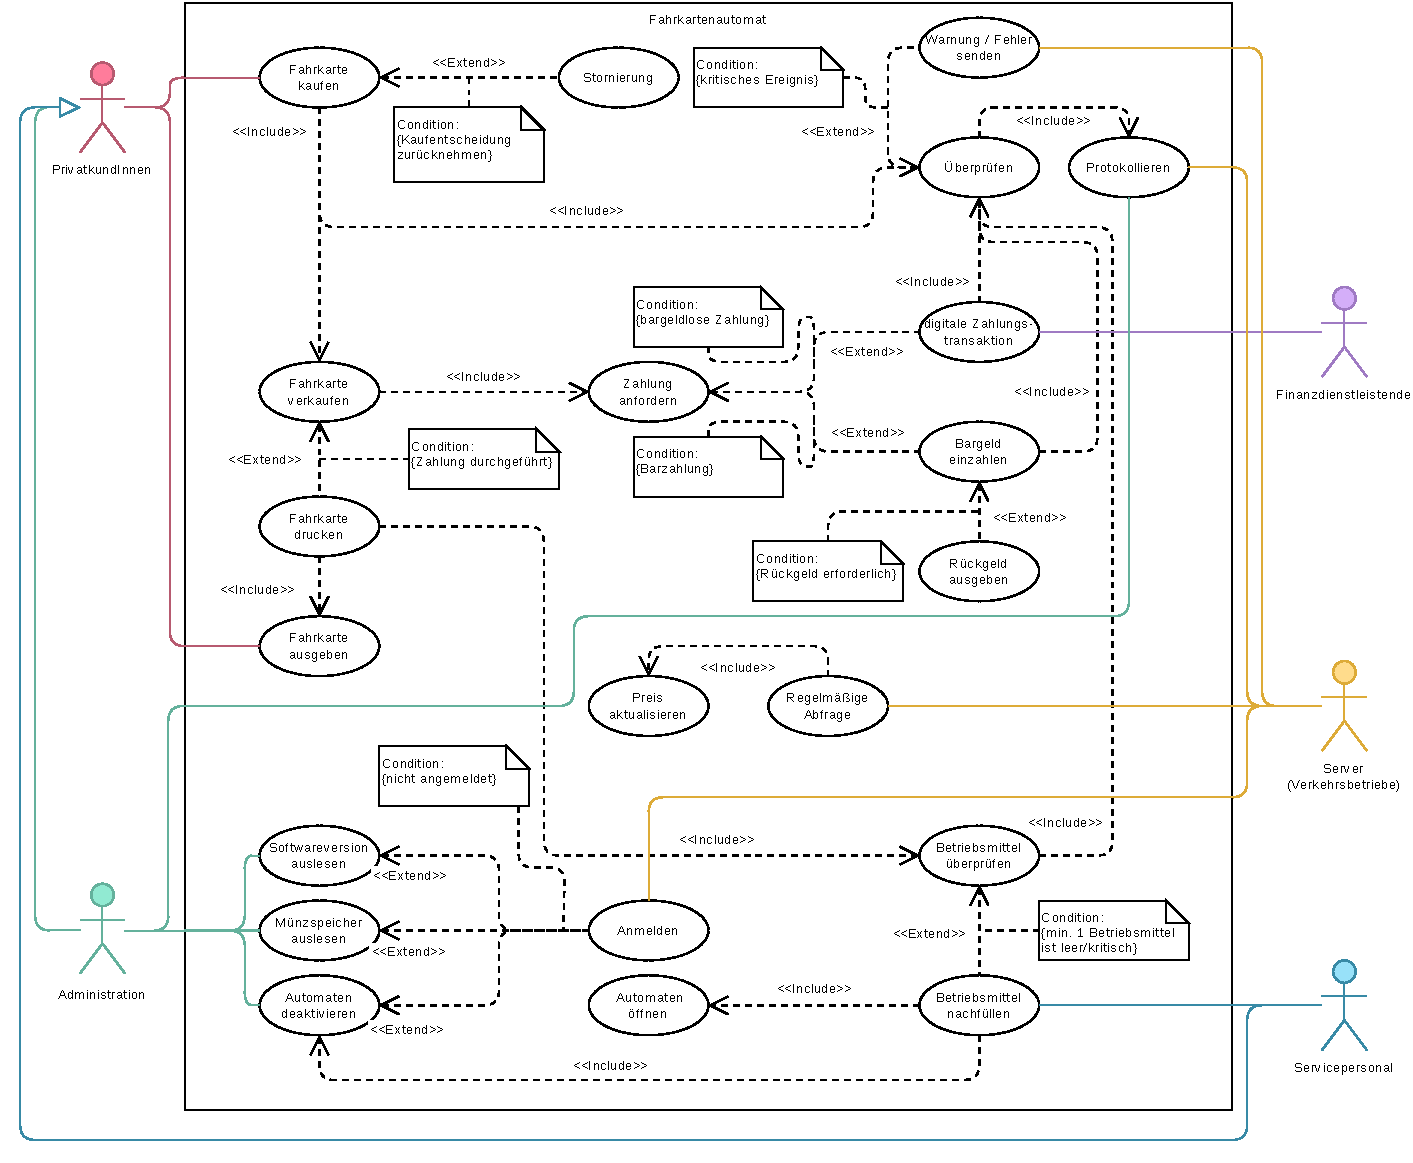
\includegraphics[width=1.7\textwidth]{use_case.pdf}}%
%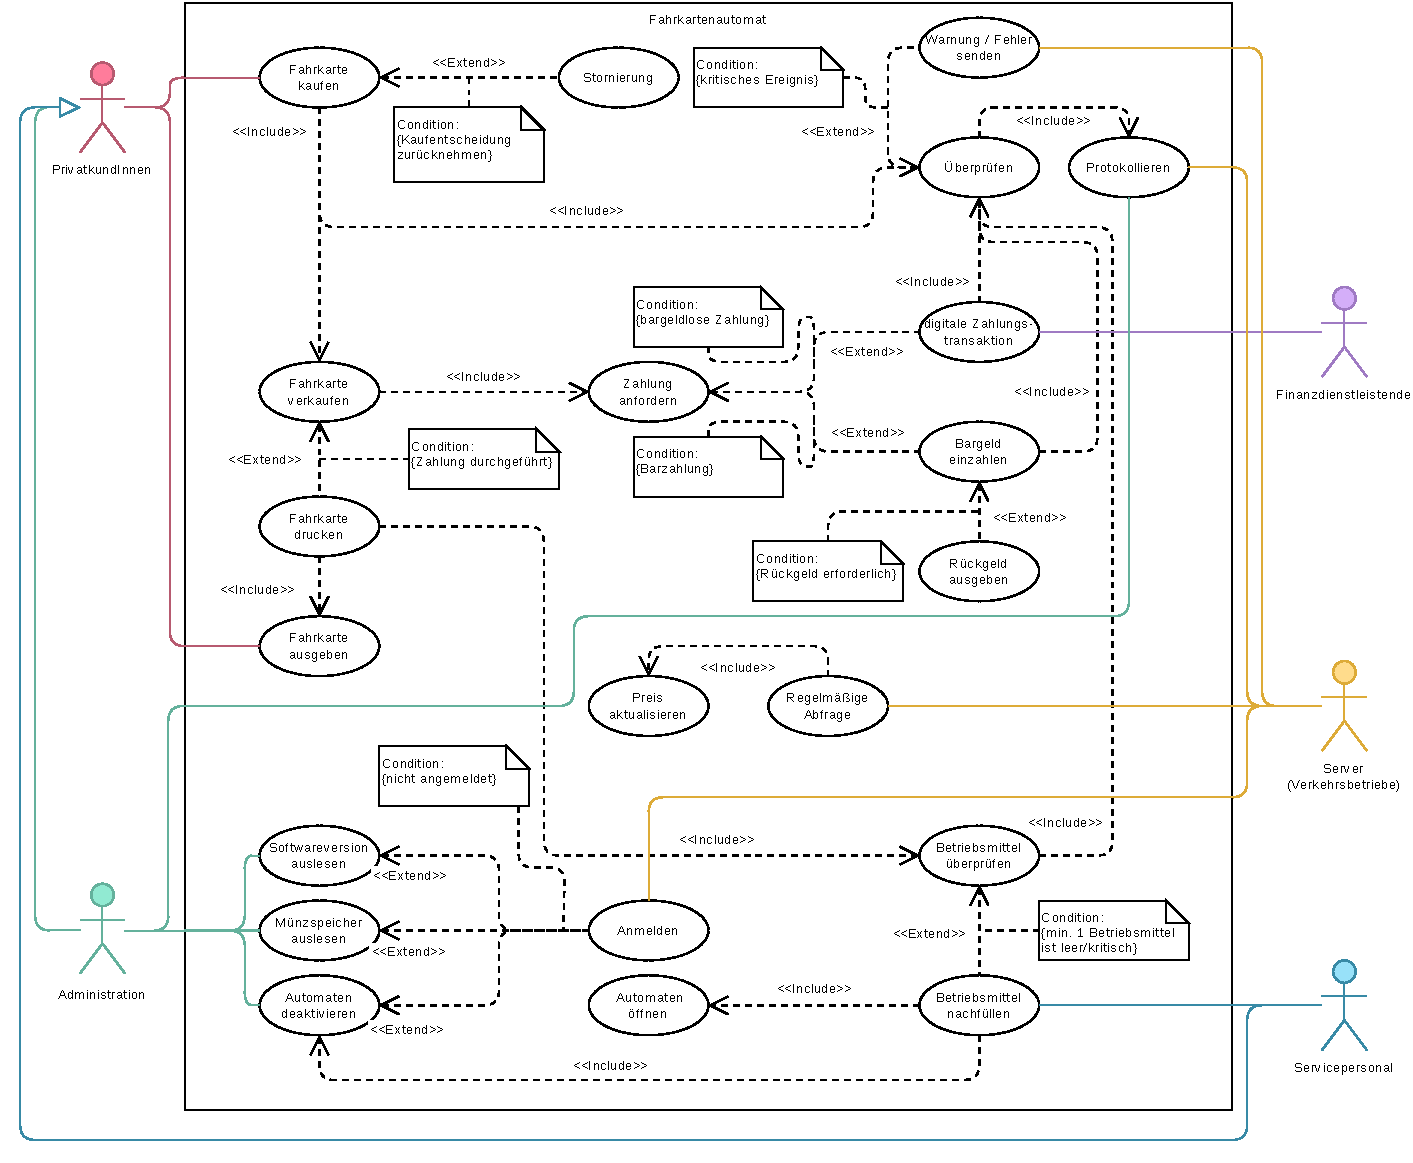
\includepdf[pages=-]{use_case.pdf}
%\end{appendices}


\end{document}